\documentclass{standalone}
\usepackage{xcolor}
\usepackage{verbatim}
\usepackage[T1]{fontenc}
\usepackage{graphics}
\usepackage{hyperref}
\newcommand{\code}[1]{\texttt{#1}}
\newcommand{\R}{R}
\newcommand{\pkg}[1]{#1}
\newcommand{\CRANpkg}[1]{\pkg{#1}}%
\newcommand{\BIOpkg}[1]{\pkg{#1}}
\usepackage{amsmath,amssymb,array}
\usepackage{booktabs}
\usepackage{multicol, calc}
\usepackage{tikz}
\usetikzlibrary{patterns,positioning,babel}
\usepackage{threeparttable}
\usepackage{natbib}
\usepackage{inconsolata}
\usepackage{listings}
\usepackage{tikz-qtree}
\usepackage{subcaption} 

\begin{document}
\nopagecolor
	
		
		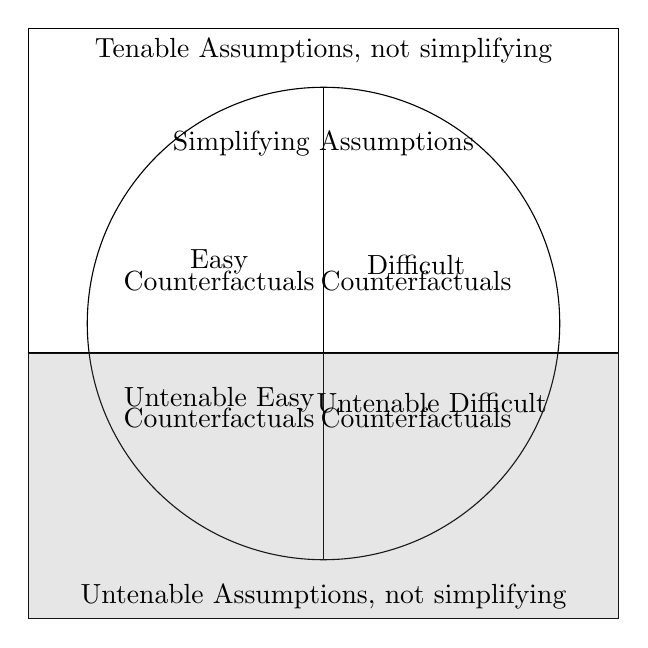
\begin{tikzpicture}[scale=2.5]
		\draw (0,0) rectangle (3,3);
		\draw (1.5,1.5) circle [radius=1.2];
		\node[above] at (1.5,2.3) {Simplifying Assumptions};
		\draw[black] (1.5, 2.7) -- (1.5,0.3);
		\draw[black] (0, 1.35) -- (3,1.35);
		\draw[fill=gray, opacity=0.2] (0,0) rectangle (3,1.35);
		\node[above] at (0.97,1.7) {Easy};
		\node[above] at (0.97,1.62) {Counterfactuals};
		\node[above] at (1.97,1.7) {Difficult};
		\node[above] at (1.97,1.62) {Counterfactuals};
		\node[above] at (1.5,0) {Untenable Assumptions, not simplifying};
		\node[below] at (1.5,3) {Tenable Assumptions, not simplifying};
		\node[above] at (0.97,1) { Untenable Easy};
		\node[above] at (0.97,0.92) {Counterfactuals};
		\node[above] at (2.05,1) {Untenable Difficult};
		\node[above] at (1.97,0.92) {Counterfactuals};
		\end{tikzpicture}
\end{document}
